\section{EnDASH - A Mobility Adapted Energy Efficient ABR Video Streaming for Cellular Networks}
From the observations in previous, we design an ABR algorithm EnDASH, which aims to reduce the energy consumption by the radio during the video streaming. EnDASH reads the environment and try to predict the future and based on the prediction it schedule segment downloading time. It does not directly schedule it, rather it change the available buffer (which is a parameter) in the player and DASH it self schedule the segment downloading according to the buffer.
\subsection{EnDASH System}
The EnDASH, first predict a expected throughput for short future ($t$) from the past and based on predicted throughput, it decides the buffer length for $t$ duration. Later on it also decides the bitrate based on the past information and current buffer length and predicted throughput.  EnDASH use three machine learning engine for each steps.

\begin{figure}[!h]
	\centering
	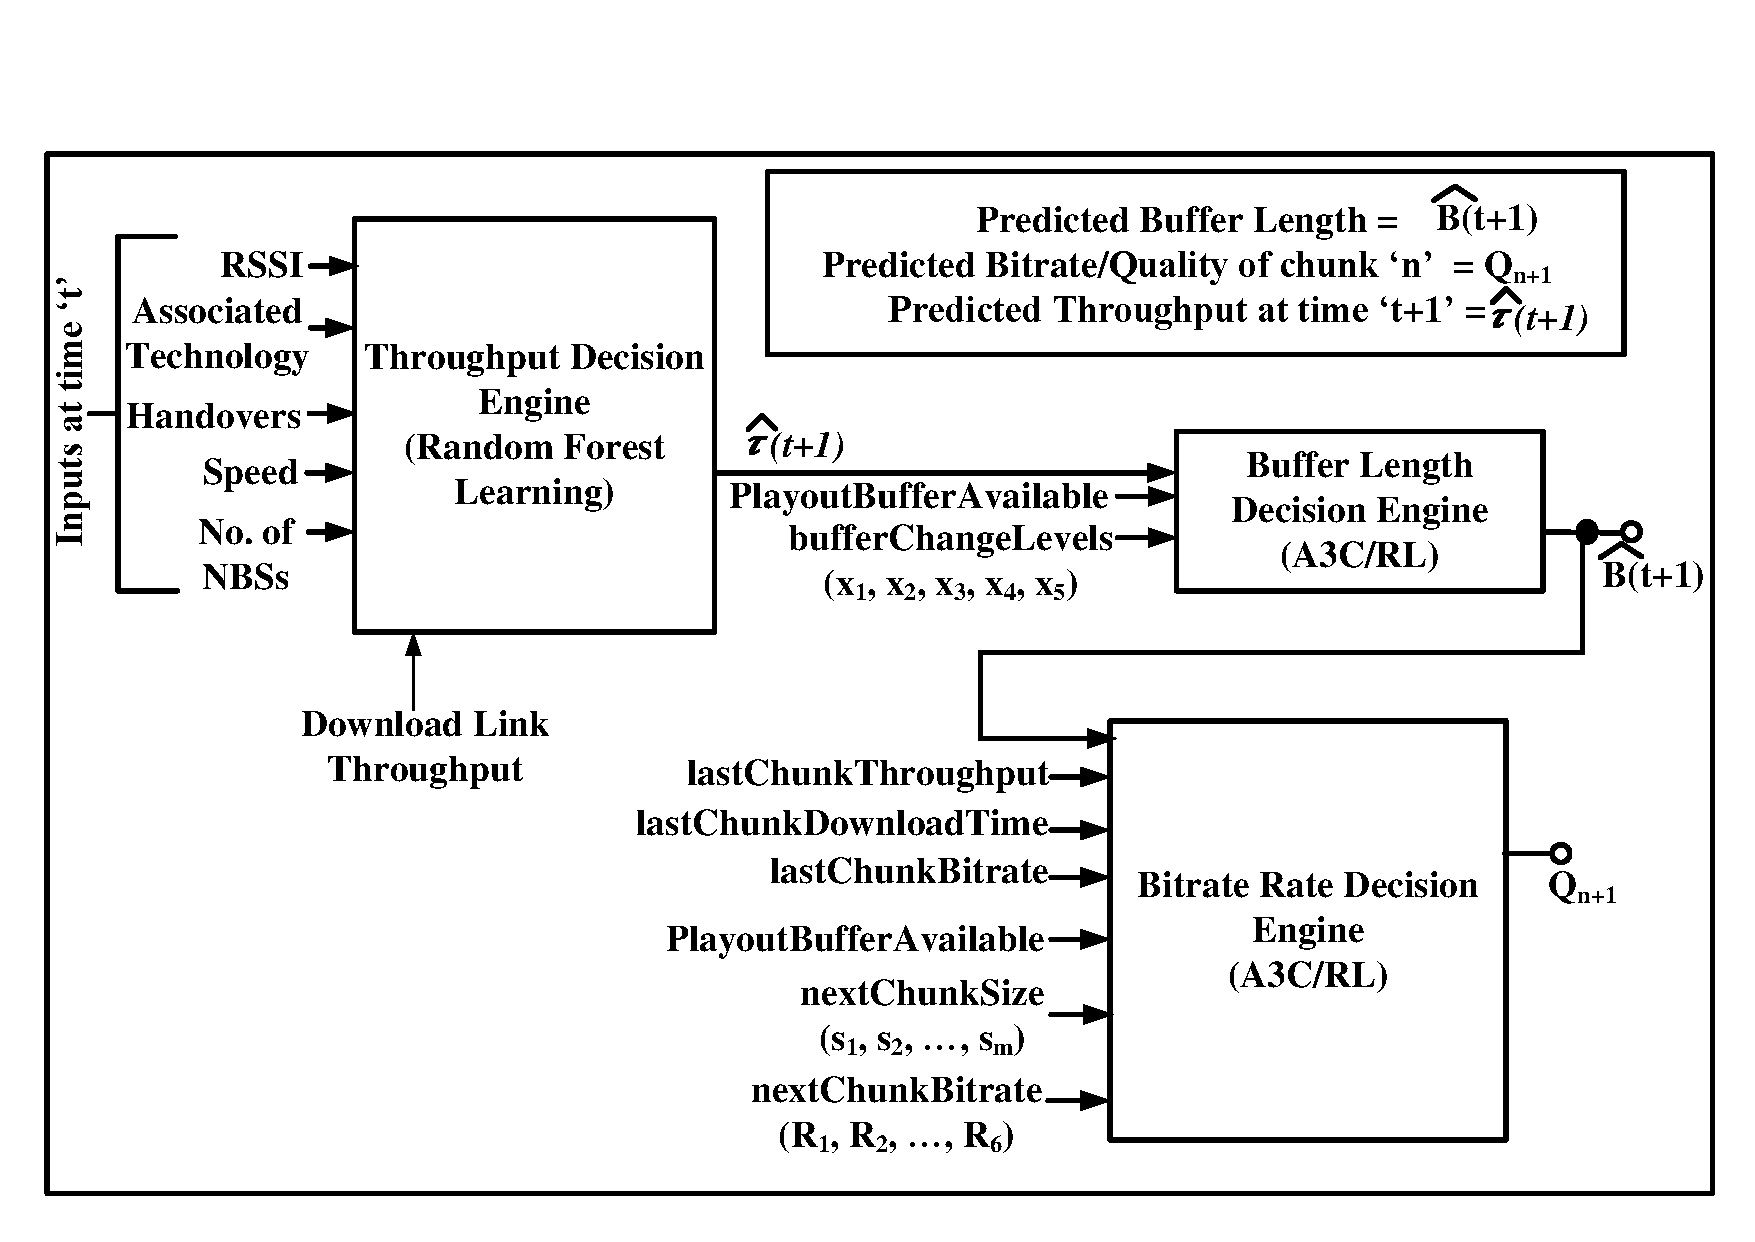
\includegraphics[width=0.7\linewidth]{img/EnDASH/EnDASH_system}
	\caption{Composite Representation of the EnDASH model; a cascaded model where the predicted throughput acts as an input network state to the Actor Critic RL based decision
engine}
	\label{fig:endash:system}
\end{figure}

\subsubsection{The throughput prediction engine}
EnDASH uses random forest learning to predict expected throughput for next 30sec from past information. It uses features like device's speed, cellular RSSI, current technology, handovers. As the features sets are huge, we feed only the $\mathrm{25^{th}}$, $\mathrm{75^{th}}$, and $\mathrm{90^{th}}$ percentile points, median and mean from its historical data of each feature.
\subsubsection{The Buffer Length Decision Engine}
The buffer length decision engine use an A3C RL based deep neural network to
determine the optimal buffer length. It takes the predicted throughput, last buffer length and possible steps to change buffer length. It returns the decision whether to buffer length needs to increase or decrease or keep same. During training phase we use a linear weighted function of energy savings with respect to a baseline ABR algorithm and the QoE score as the reward.

The throughput prediction engine and buffer length prediction engine runs only once in every $t$ time in these order only.
\subsubsection{The Bitrate Decision Engine}
EnDASH use another A3C RL based deep neural network to estimate the quality of next chunk based on several playback related players and the buffer length similar to the parameters used in the Pensieve\cite{mao2017neural}. It runs before fetching the next segment and uses QoE as the reward during the traing phase.

Complete architechtue is presented in the Fig.~\ref{fig:endash:system}.

\begin{figure}[!h]
	\begin{minipage}[t]{0.48\linewidth}
		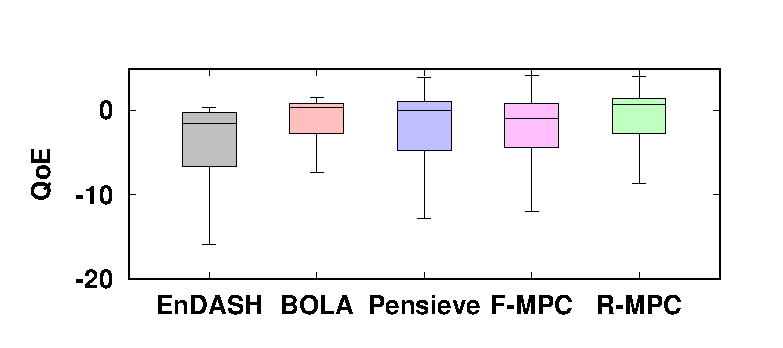
\includegraphics[width=\linewidth]{img/EnDASH/QoE}
		\caption{\label{fig:endash:qoe}}
	\end{minipage}\hfill
	\begin{minipage}[t]{0.48\linewidth}
		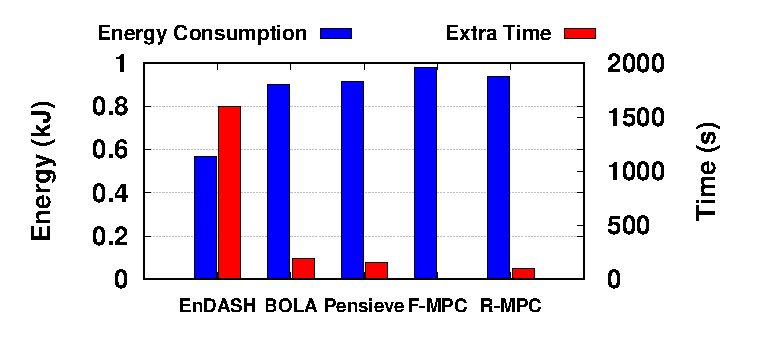
\includegraphics[width=\linewidth]{img/EnDASH/EnergyConsumption}
		\caption{\label{fig:endash:energy}}
	\end{minipage}
\end{figure}
\subsection{Evaluation}
We trained and test all these three engines in a emulation platform from the data we collected from comodity smartphones like Moto G5, Micromax canvas over Airtel, Reliance Jio and Vodaphone. Once training and testing completed for each individual modules, we run experiment in our emulation based test bed, where we compare QoE performance and energy saving of EnDASH. In Fig.~\ref{fig:endash:qoe} we compare the performance in terms of QoE with modern ABR algorithms. EnDASH slightly compromizes the QoE, however, it save lot of energy. In Fig.~\ref{fig:endash:energy}, we plot the energy uses and possible run time with respect Fast-MPC, and it turns out that video can be played for another 20-25 minutes with EnDASH compared to Fast-MPC.
